
\subsection{Overview}
In distributed systems and HPC, resource usage are typically monitored to detect any hardware and software issues. Real-time monitoring applications help provide sustain and consistent services and engage performance of their system. Distributed systems were built with complex hardwares and require to incorporate with various hardwares such as router, switch, network, and servers along with computing resources like cpu, memory and disk. In Cloud Computing, people have attention to monitoring and accounting systems in virtualized environments, so that they can measure resource consumption which is what they are paying for on the on-demand service, cloud computing. 

Many places now adopt virtualization and cloud services to enhance the capacity of their system infrastructure and performance. Performance management is getting more important in this regard for identifying and delivering reasonable resource allocation. But traditional performance software are still designed to measure a certain type of resources and system administrators raised needs for a unified performance management with virtual resource allocation which provides a bird eye's view to monitor system utilization with the proper provision and allocation of resources~\cite{Habibzai12}. The unified monitoring software is not only about an integrating metric units and aggregating numerical values but also about making sure that the applications on the services are efficiently consuming allocated resources and the resources are properly allocated in the right place at the right time. Understanding system utilization and application performance with the observation from the software is important to satisfy service-level agreements (SLAs) and improve the system administration, however in a virtualized environment, measuring shared resources is not an easy task since they are in multiple points and different layers. 



\subsection{Real Consumption vs Allocation}
There are two types of measuring resource usage on the cloud. Like a conventional monitoring, resource consumption on the cloud is based on current usage data for cpu, memory, network and disk traffics. These are dynamically changing according to traffics, and are important to validate system health frequently. The other type of measuring resource usage is measuring the amount of allocated resources. It is an accounting system that records allocation of resources. In a shared resource environment which is a fundamental concept in utility computing, the amount of allocated resource means that your requested resource will be dominated to you not interrupted by any other users. Resource allocation is not measuring real-time resource usage. Instead, it records rented resources in an accounting book for billing and charging. There are static metrics for allocation such as allocated number of cpu cores, memories, and disks. Number of public IP addresses is also counted for metrics.

 
\subsection{Design} \label{S:design}

CloudMetrics pursues to provide an integrated accounting service which users and system administrators are able to obtain cloud usage data for various cloud platforms such as Eucalyptus, OpenStack, and Nimbus and so on. The usage information will cover several aspects like billing, auditing, monitoring, and accounting systems. Parsing log files is a main process for collecting and storing information regarding the utilization of virtual machine (VM) instances and service nodes or clusters. The current development focuses on:

\begin{itemize}
 \item A measuring tool of resource used
 \item A command-line interface to explore the cloud usage data
 \item A visualization to help understand usage data
 \item A RESTful API Service to support external services
\end{itemize}


\begin{comment}
\begin{figure*}[htb] 
\begin{center}
    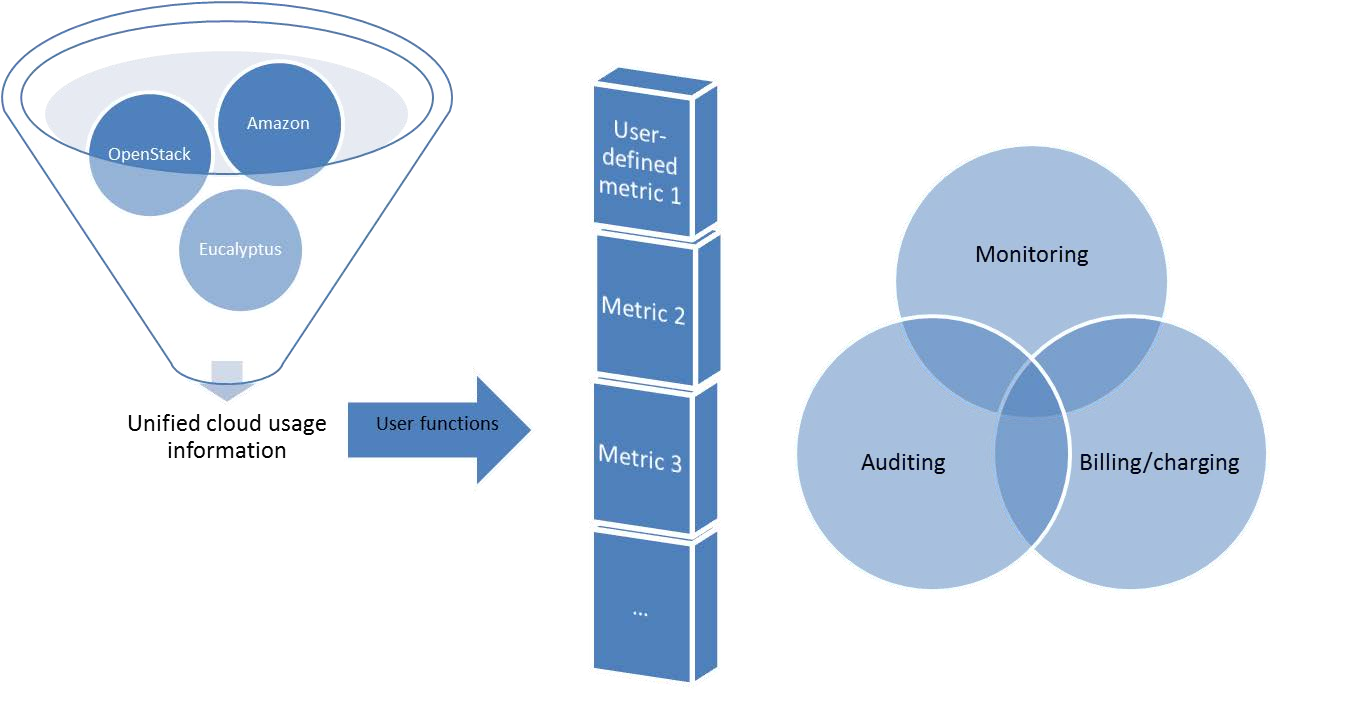
\includegraphics[width=1.0\textwidth]{images/Picture1.pdf} 
\end{center}
  \caption{ NOT SHOWN Overview of CloudMetrics \hyungro{we need to redraw as
      color scheme is not so good for reproduction. what is original
      file? I hope this is pptx? Maybe this picture is not that
      important as contained already in architecture drawing? bu we do
    not see there auditing, monitoring, billing, as well as defining and
  adding new metrics. customization is something we missed in introduction.}}\label{F:fig1} 
\end{figure*} 
\end{comment}

%CloudMetrics consists of four components: 1) a measuring tool of resource allocation  and 2) a CLI tool to define metrics and collect usage data 3) a visualization tool to provide graphical representative of the data and 4) Web Service APIs to support other applications e.g. scheduling and dynamic provisioning. We have the log parser named by fg-log-parser which reads and examines log messages of IaaS platforms (e.g. Eucalyptus, OpenStack) to collect metrics and stores the metrics into a database using a global object i.e. JSON converted from a python dictionary data type. fg-metrics takes the role of analyzing usage data and generating results in a image file or a csv file. We assume every measured data is stored in the database from five different resources (Foxtrot, Hotel, India, Sierra, Alamo) to support more than 400 projects and 3200 members as of 2014. Our new development of federation management, CloudMesh, uses the REST APIs to deliver accounting features on its command-line interfaces and web services~\cite{cloudmesh14}.

\begin{table}[htb]
  \caption{New accounts in FutureGrid}
\begin{scriptsize}
\label{T:tab00}
  \begin{tabular}{l|c|c}
   Year & Users & Projects \\
   \hline
   2011 & 637 & 100 \\
   2012 & 900 & 114 \\
   2013 & 614 & 103 \\
 \end{tabular}\\
\end{scriptsize}
 \end{table}

 \begin{table}[htb]
   \caption{Active Users in Cloud, HPC or Both}
\begin{scriptsize}
\label{T:tab000}
   \begin{tabular}{l|c|c|c}
     Year & Cloud & HPC & Both \\
     \hline
     2011 & 134 (123) & 154 (120) & 33 (26) \\
     2012 & 195 (130) & 164 (122) & 183 (144) \\
     2013 & 235 (140) & 200 (133) & 70 (38) \\
   \end{tabular}\\
   $^*$ New users shown in parenthesis
\end{scriptsize}
 \end{table}


 In average, FutureGrid accepted more than 100 projects every year, and around 60 to 90 members participated in each project. In table~\ref{T:tab000}, we noticed that more user were getting used both Cloud and HPC over the years instead of only using either Cloud or HPC. It implies that Cloud and HPC together can be beneficial to users.


\begin{comment}

\subsection{Pricing Comparison}

Comparing pricing of the cloud is complicated and may lead to false analogy because each cloud provider offers various services with different performance. The pricing comparison, however, is important when people start to consider adopting cloud services among a lot of selections from different providers. In the comparison, important criteria are revealed through its pricing table. For example, there are a range of service offered, a size of available systems, costs, discounts and benefits such as technical support, and development tools. Amazon AWS, Windows Azure, Google Compute Engine (GCE), HP Cloud, IBM and Rackspace are compared. Pricing is scenario based. It can't be simply compared with numbers. GCE looks cheaper than other competitors, but others have several options to reduce cost. For example, a pay-ahead model provides a discount for same instances, and a spot instance also provides a way of saving entire cost for task intensive workloads in a small amount of time. In Table~\ref{T:tab0}, different price tags for virtual machine instances are described. With the comparison of the smallest vm instance which is 1 virtual core, 600-768MB memory and no storage option, we can see most IaaS service providers have similar pricing charts.

\begin{table}[htb]

%\caption{Pricing chart for instances from AWS, GCE, and Azure \newline * China (Beijing) region will be available in early 2014, and GovCloud region is also included.}\label{T:tab0}

 
\caption{Pricing chart for instances from AWS, GCE, and Azure}\label{T:tab0}
%\begin{footnotesize}
%\begin{tabular}{l|p{2.5cm}|l|p{2cm}}
 %    &  \shortstack{Billing\\ granularity} &   Price & \shortstack{Price\\ Variation} \\
 % \hline
%AWS &   By hour & \$0.02 &      \shortstack{10 regions*,\\ 6 platforms} \\
%GCE &   By minute$^1$ &       \$0.019  &      \shortstack{2 regions\\ (US, Europe)} \\
%Azure & By minute$^2$ & \$0.02 &    \shortstack{6 regions,\\ 5 platforms} \\
%\end{tabular}\\
%$^1$ with a minimum of 10 minutes\\
%$^2$ with a no minimum and free of charge for less than 5 minutes
\end{table}

\subsubsection{Example of Pricing Comparison}

We tried to apply each pricing model; Amazon AWS, Google Compute Engine, Microsoft Azure; to the usage data of the class (P434 distributed systems at Indiana University), to compare cost estimate of cloud resources. Google Compute Engine is the least expensive and 16\% lower than Amazon AWS. It is mostly because of that Google has 10\% discount pricing chart compared to AWS. We observed that a minute basis charge is only 3.3\% less expensive for this class. Some restrictions and offers such as Google's 10-minute minimum charge and Azure's less 5-minute free of charge are relatively small amount of a discount or an extra charge. Google's 10-minute minimum charge asks 0.18\% extra charge to the class, Azure provides 0.05\% discount through their less 5-minute free of charge. Amazon only has an hourly based pricing model, while Google Compute Engine and Windows Azure offer a minute basis charge for use of virtual machine instances. Three types of instances (small/medium/large) had been used for its coursework and projects and usage of virtual machine instances was only calculated without network and storage usage. Table~\ref{T:tab1}, ~\ref{T:tab2} shows pricing comparison to the class.

\begin{table}[htb]
\caption{Usage data to the class}
\begin{scriptsize}
\label{T:tab1}
\begin{footnotesize}
\begin{tabular}{l|r|l|l|r|r}
\shortstack{Instance\\types} & \shortstack{Instan-\\ces} & \shortstack{Charge\\by hour} & \shortstack{Charge\\by min} & Google$^1$ & Azure$^2$ \\
  \hline
small & 165 & 37,140 & 29,622 & 29,875 &29,582 \\
medium & 6 & 16,080 & 15,891 & 15,891 & 15,891 \\
large & 490 & 649,860 & 629,969 & 631,047 & 629,667 \\
  \hline \hline
Total & 661 & 703,080 & 675,482 & 676,813 & 675,140 \\
\end{tabular}\\
$^1$ includes 10~min minimum charge\\
$^2$ includes 5~min free charge
\end{footnotesize}
\end{scriptsize}
\end{table}

%* Instance types are not same. Chosen by a similarity of vCPU and Memory
%** Captured by January, 2014

\begin{table}[htb]
\caption{Pricing comparison to the class}
\begin{scriptsize}
\label{T:tab2}
\begin{footnotesize}
\begin{tabular}{l|l|l|l|l|l|p{2cm}|}
Service & Cost & \multicolumn{3}{|c|}{Price per hour} \\
  & Estimate &  Small& Medium& Large \\
 \hline
AWS$^1$ & \$2,668.74  & \$0.06 & \$0.12 & \$0.24 \\
GCE$^2$ & \$2,231.54  & \$0.054 & \$0.104 & \$0.207 \\
Azure$^3$ & \$2,580.03  & \$0.06 & \$0.12 & \$0.24 \\ 
\end{tabular}
\\
\\
$^1$US East, Linux, charged 1 hour if runtime is <1 hour\\
$^2$US, Linux, charged 10 minutes if runtime is <10 minutes\\
$^3$Linux, charged by minute but free is <5 minutes\\
\end{footnotesize}
\end{scriptsize}
\end{table}

\end{comment}


% scheduling

%In a sense of security, accounting is also able to provide some information for investigation of suspected security intrusions not only providing resource usage1 monitoring. Billing is another purpose of accounting.



% \begin{sidewaystable*}
% \caption{table 3}\label{T:tab3}
% 
% \begin{footnotesize}
% \begin{tabular}{|p{2cm}|p{2cm}|p{1.5cm}|p{1.5cm}|p{2cm}|p{1cm}|p{1.5cm}|p{2cm}|p{2cm}|p{2cm}|}
% \hline
% Provider & Charging & Cost 1vCPU/hour    & Cost 1GB/hour & OS & Max vCPU & Memory min - max &\# of instance types & Discount program & Free allowance\\
% \hline
% \hline
% Aws & hourly & \$0.04  & \$0.02  & Linux & 32 & 615MB - & 22 & spot instance;  & \$100 for educators and student\\
%     &              &         &         & Windows +14-56\%     &    & 244GB    &       & reserved instances & Grant for researcher, AWS educated grant program\\
%     &              &         &         & Asia + 25\%          &    &                 &       &                    & \\
% \hline
% Google Compute Engine & 10 minutes + & \$0.08  & \$0.01  & Linux (Debian; CentOS) & 16 & 600MB - & 1- & n/a & Google app reward programs\\
%  & every minute after that &  &  & (RHEL; SUSE premium operating systems) *** &  & 104GB & (4 high cpu + 4 high memory + 2 small + 5 standard) &  & \$1000 for educator\\
%  &  &  & Europe + 4.5\% - 27\%  &  &  &  &  &  & \$60;000 for research project\\
% \hline 
% IBM CloudLayer (by Softlayer) & monthly & \$0.50  & varies & Linux;  & 16 & 1GB  & Build your own cloud server offers customized options &  & one month trial for 1 vcpu + 1gb memory + 25 storage\\
% \hline
%  & hourly & to &  & Windows + \$0.05 to &  & -  &  &  & \\
%  &  & \$0.10  &  &               \$0.10 / hour &  & 64GB &  &  & \\
% \hline 
% HP cloud & hourly & \$0.02  & \$0.02  & Linux; Windows; SUSE & 16 & 1GB  & 11 (8 standard + 3 memory intensive) &  & \$300 free trial for 90 days (\$100 for each month)\\
%  &  &  &  & (windows: 10-200\% extra charge; &  & -  &  &  & \\
%  &  &  &  & SUSE: 4\% - 200\% extra charge) &  & 120GB &  &  & \\
% \hline 
% Microsoft Azure & Free first 5 minutes & \$0.05  & \$0.02 (approx.) & Linux;  & 8 & 768MB -  & 8 (A0-A7) & 6-Month; 12-month pre-pay membership & \$200 free trial of first month\\
%  &  &  & Windows is expensive 30-50\% more than linux & Windows + 30-50\%  &  & 56GB &  &  & \\
% \hline 
% Rackspace & minute &  & varies & Linux; Windows, (windows: 25\% extra charge) & 32 & 1GB - 120GB  & 9 & Volume discount (4\% to 20\% for spending over \$5;000 - \$ 10; 000 per month; 8\% for \$10;001 - 30;000; 12\% for \$30;001 - \$50;000) Commitment discount (4\% to 40\%) Prepayment discount with commitment (7\% to 55\%)& \$300 developer discount (\$50 each for six months)\\
% \hline
% \end{tabular}
% \end{footnotesize}
% \end{sidewaystable*}
% 
% 
% Provider      Charging        Cost
% 1 vCPU /hour  Cost
% 1 GB
% /hour OS      Max vCPU        Memory min - max        \# of instance types    Discount program        Free allowance
% Aws
%       hourly  \$0.04
%       $0.01927        Linux
% Windows +14-56% 
% Asia + 25%    32      615MB -
% 244GB 22      spot instance, 
% reserved instances    $100 for educator's student
% Grant for researcher
% AWS educated grant program
% Google Compute Engine 10 minutes +
% every minute after that       $0.0788
%       $0.006636
% 
% Europe + 4.5% - 27%   Linux (Debian, CentOS)
% (RHEL, SUSE premium operating systems) ***    16      600MB -
% 104GB 15
% (4 high cpu + 4 high memory + 2 small + 5 standard)   n/a     Google app reward programs
% $1000 for educator
% $60,000 for research project
% IBM CloudLayer (by Softlayer) monthly
% hourly        $0.5
% to
% $0.10 varies  Linux, 
% Windows + $0.05 to
%               $0.10 / hour    16      1GB 
% – 
% 64GB  Build your own cloud server offers customized options           one month trial for 1 vcpu + 1gb memory + 25 storage
% HP cloud      hourly  $0.015  $0.015  Linux, Windows, SUSE
% (windows: 10-200% extra charge,
% SUSE: 4% - 200% extra charge) 16      1GB 
% – 
% 120GB 11 (8 standard + 3 memory intensive)            $300 free trial for 90 days ($100 for each month)
% Microsoft Azure       Free first 5 minutes
%       $ 0.05  $0.02 (approx.)
% Windows is expensive 30-50% more than linux   Linux, 
% Windows + 30-50%      8       768MB – 
% 56GB  8 (A0-A7)       6-Month, 12-month pre-pay membership    $200 free trial of first month
% Rackspace     minute          varies  Linux, Windows
% (windows: 25% extra charge)   32      1GB – 
% 120GB 9       Volume discount (4% to 20% for spending over $5,000 - $ 10, 000 per month, 8% for $10,001 - 30,000, 12% for $30,001 - $50,000)
% Commitment discount (4% to 40%)
% Prepayment discount with commitment (7% to 55%)       $300 developer discount ($50 each for six months)

\task{We can think about rerouting VM instances to ensure scalable services by avoiding crowded zone. This cloud shifting may support relaxed management regarding load balancing of the cloud systems. The other potential work is probably that we can provide an indicator of cost-efficient leasing on the cloud based on the correlation data measured by this activity. Cost of using cloud can be reduced in many ways, including finding inexpensive cloud service providers, and using parallel processing technique such as MapReduce. Measuring correlation between physical and virtual resources could mean that we can find a spot in which reliable performance is guaranteed and it would be one of the main techniques to provide cost-efficient cloud renting across all the resources.}


\section{conlcusion}

This activity provides a way of understanding performance and resource utilization across system and application layers, especially on cloud resources. With the various requests of resource allocation on the cloud, project leaders and members encounter challenges with finding availability of virtual resources and handling this information. Cloud users in a pool of shared resources can suffer performance degradation by other users. Monitoring physical resources is not enough to mitigate this degradation in cyberinfrastructure. In this paper, Cloud Metrics offer several means to get information of resource utilization and performance. In addition, the classification of performance managements and case studies provide an inside visibility to help identify the issues easily and finding solutions regarding resource allocation on the cloud. To enhance performance of systems and get powerful machines, understanding resource allocation of virtual resources is needed to avoid under performing systems and applications.


\begin{comment}
\subsubsection{Keeneland}

Keeneland project is a high performance computing system to support GPU development with commodity linux clusters led by the Georgia Institue of Technology in collaboration with the University of Tennessee at Knoxville and Oak Ridge National Laboratory. Two phases were available in the project.  Keeneland Initial Delivery System (KIDS) consisted of Intel Xeon X5660 240 CPUs and Nvidia Tesla M2090 360 GPUs to support scientific and engineering applications with the total peak performance of 255 TFLOPS. The Keeneleland Full Scale System (KFS) provided bigger computing resources with 264 HP nodes by two 8-core Intel Xeon E5 CPUs, for a total of 528 CPUs and 792 Nvidia M2090 GPUs. KFS was used in XSEDE with the peak performance of 615 TFLOPS~\cite{keeneland}\cite{keeneland-xsede}.

\subsubsection{Darter}

Darter is a supercomputer supported by the University of Tennessee, Knoxville and the National Institute for Computational Sciences (NICS) with 724 compute nodes on a Cray XC30 (Cascade) system and Lustre file system for a total of the peak performance of 240.9 Tflops~\cite{darter-nics}.  \end{comment}

\subsubsection{Stampede}

Stampede is a supercomputer supported by the Texas Advanced Computing Center (TACC) for open sicence research. Stampede provides the total peak performance of 9.6 Petaflops with 6400 nodes and 14 Petabytes disk sizes~\cite{stampede-tacc}.




\begin{tikzpicture}[grow'=right,level distance=1.25in,sibling distance=.25in]
\tikzset{edge from parent/.style= 
           {draw, edge from parent fork right}}

    \begin{dot2tex}[dot,tikz,codeonly,styleonly]
        digraph G  {
	     user -> "IT Personal"
	     user -> "Funder"
        }
    \end{dot2tex}
\end{tikzpicture}

\begin{dot2tex}[tikz]
digraph G {
  rankdir="LR";
  ranksep=0.01;
  nodesep=0.01;  
node [shape="none"];
user -> "IT Personal" -> a
user -> Funder
}
\end{dot2tex}

\begin{dot2tex}[tikz]
digraph Orthogonal {
 rankdir="LR";
 graph [label="Orthogonal edges", splines=ortho, nodesep=0]
 node [shape=box]
 user -> {IT Personal Funder}
}
\end{dot2tex} 


\begin{small}
\begin{tikzpicture}[grow'=right,level distance=1.25in,sibling distance=.25in]
\tikzset{edge from parent/.style= 
           {draw, edge from parent fork right}}
\Tree 
   [. user 
       [.{IT personal} ]
       [.{Funder} ] 
   ]
\end{tikzpicture}
\end{small}


\begin{comment}
  \begin{forest}
%for tree={
%    edge path={\noexpand\path[\forestoption{edge}] (\forestOve{\forestove{@parent}}{name}.parent anchor) -- +(0,-12pt)-| %(\forestove{name}.child anchor)\forestoption{edge label};}
%}
    for tree={grow'=east, child anchor=west, anchor=base
     west, tier/.pgfmath=level()}
    [Root,
    [C1
    [GC1Long [GGC1][GGC2]]
    [GC2 [GGC1][GGC2Long]]
    ]
    [C2Long,
    [GC1 [GGC1][GGC2]]
    [GC2]
    ]
    [C3VeryLong
    [GC1][GC2]
    ]
    ]
  \end{forest}

\end{comment}


\begin{comment}

  \begin{comment} 

    Abstract

    In shared resource environments, usage data is necessary to identify utilization of the infrastructure by users. Many cloud platforms recently started to collect measurements for use of resources that can be applied to billing and monitoring. Understanding utilization and performance through these measurements is crucial in the infrastructure in order to provide better cloud provisioning, system management and capacity planning. In this paper, we present an integrated cloud accounting solution applicable to federated cloud environments. We have tested this framework on FutureGrid.  Our system is integrated as a CloudMetric component into a larger framework called cloudmesh that targets explicit user or administor controlled federation of clouds.  Our cloudmesh CloudMetrics component is ablehich is an XSEDE resources. Based on the observation on FutureGrid, we found that different patterns between scientific research projects and educational projects regarding the type of virtual machines (VMs) and the patterns of using virtual resources.  CloudMetrics enables users and project leaders to identify utilization and performance.

\end{comment}

\section{OLD ABSTRACT} 

In shared resource environments, usage data is necessary to identify utilization of the infrastructure by users. Many cloud platforms recently started to collect measurements for use of resources that can be applied to billing and monitoring. Understanding utilization and performance through these measurements is crucial in the infrastructure in order to provide better cloud provisioning, system management and capacity planning. In this paper, we present an integrated cloud accounting solution, Cloud Metrics, to measure cloud resource usage across several cloud platforms such as OpenStack, Nimbus, and Eucalyptus. The usage data allows a user to see as how all resources are efficiently supplied to their applications and discover patterns from cumulative data. With Cloud Metrics, virtual resources such as compute, storage and network are measured to evaluate time and cost of user applications and the statistics for these resources offer visibility to utilization of cloud resources. This article shows statistical analysis of several case studies by tracing resource allocation on FutureGrid. Based on the observation on FutureGrid, we found that different patterns between scientific research projects and educational projects regarding the type of virtual machines (VMs) and the patterns of using virtual resources. Cloud Metrics enables users and project leaders to identify utilization and performance.

\todo[inline]{remove old abstract, but read if there is info we need
  to maintain.}
\end{comment}


%\begin{forest} 
% for tree={grow'=east, child anchor=west, anchor=base
%      west, tier/.pgfmath=level()}
%[VP
%[DP] [V
%[V]
%[DP] ]
%] \end{forest}




